\documentclass[12pt,a4paper]{article}
\usepackage[spanish]{babel}
\usepackage[utf8]{inputenc}
\usepackage{graphicx}
\usepackage{float}
\usepackage{amsmath}
\usepackage{geometry}
\usepackage{fancyhdr}
\usepackage{hyperref}
\geometry{margin=2.5cm}

\hypersetup{
    colorlinks=true,
    linkcolor=blue,
    urlcolor=blue
}

%--------------------------------------------------
% PORTADA
%--------------------------------------------------
\begin{document}

\begin{titlepage}
\centering

{\huge\bfseries Aplicación de Búsqueda Informada A* al Robot Aspiradora (PEAS)\par}
\vspace{1.5cm}
{\Large Inteligencia Artificial\par}
\vspace{1cm}
{\Large Autor: \textbf{Aaron Rodrigo Ramos Reyes}\par}
\vspace{0.5cm}
{\large Fecha de entrega: 29 de Octubre de 2025\par}
\vfill
{\large \textit{Tarea 2 – Punto B: Aplicación de A* sobre modelo PEAS.}\par}
\vspace{1cm}

\end{titlepage}

%--------------------------------------------------
% INTRODUCCIÓN
%--------------------------------------------------
\section{Introducción}

En esta parte del trabajo se aplica el algoritmo de búsqueda informada \textbf{A* (A-star)} al agente \textbf{robot aspiradora inteligente}, de acuerdo con el modelo \textbf{PEAS} descrito en la tarea anterior.

El entorno se modela como una \textbf{cuadrícula de celdas} donde existen:
\begin{itemize}
    \item Celdas libres (transitables).
    \item Celdas ocupadas por muebles (bloqueadas).
    \item Celdas sucias que el robot debe limpiar.
\end{itemize}

El robot se mueve en cuatro direcciones (arriba, abajo, izquierda, derecha) sin diagonales, y su objetivo es limpiar todas las celdas sucias de acuerdo con dos modos de funcionamiento:
\begin{enumerate}
    \item \textbf{Modo rápido:} Minimiza el tiempo total de limpieza, buscando la distancia Manhattan más corta posible.
    \item \textbf{Modo eficiente:} Minimiza el consumo energético, penalizando los giros innecesarios y movimientos redundantes.
\end{enumerate}

Ambos modos son simulados visualmente mediante la librería \textbf{pygame}, donde se observa el recorrido del agente en tiempo real.

%--------------------------------------------------
% MODELO PEAS DEL ROBOT ASPIRADORA
%--------------------------------------------------
\section{Modelo PEAS del agente}

\begin{itemize}
    \item \textbf{Performance (Desempeño):}
    \begin{itemize}
        \item Minimizar el tiempo total de limpieza.
        \item Minimizar el consumo energético (número de movimientos y giros).
        \item Limpiar todas las celdas sucias sin chocar con muebles.
    \end{itemize}

    \item \textbf{Environment (Entorno):}
    \begin{itemize}
        \item Cuadrícula de tamaño $N \times N$ (en este caso $8\times8$).
        \item Celdas pueden ser:
        \begin{itemize}
            \item 0 – Libre.
            \item 1 – Mueble (obstáculo).
            \item 2 – Sucia (debe ser limpiada).
        \end{itemize}
        \item Posición inicial aleatoria del robot.
    \end{itemize}

    \item \textbf{Actuators (Actuadores):}
    \begin{itemize}
        \item Moverse arriba, abajo, izquierda o derecha.
        \item Aspirar (limpiar) la celda actual.
    \end{itemize}

    \item \textbf{Sensors (Sensores):}
    \begin{itemize}
        \item Detectar si la celda actual está sucia.
        \item Detectar si una celda vecina contiene un obstáculo.
        \item Detectar su posición dentro de la cuadrícula.
    \end{itemize}
\end{itemize}

%--------------------------------------------------
% DESCRIPCIÓN DEL ALGORITMO A*
%--------------------------------------------------
\section{Algoritmo A* aplicado}

El algoritmo A* busca la ruta óptima entre dos celdas mediante la función:
\[
f(n) = g(n) + h(n)
\]
donde:
\begin{itemize}
    \item \( g(n) \): costo real desde el inicio hasta el nodo actual.
    \item \( h(n) \): heurística estimada desde el nodo actual al objetivo (distancia Manhattan).
\end{itemize}

En el contexto del robot:
\begin{itemize}
    \item \( g(n) \) incluye penalizaciones adicionales según el modo:
    \begin{itemize}
        \item Modo rápido: \( g(n) = 1 \) (cada movimiento cuesta 1 unidad).
        \item Modo eficiente: \( g(n) = 1 + 1.5 \) si hay cambio de dirección (penaliza giros).
    \end{itemize}
    \item \( h(n) = |x_1 - x_2| + |y_1 - y_2| \)
\end{itemize}

El algoritmo se repite para limpiar todas las celdas sucias. Cada vez que el robot llega a una celda sucia, la limpia y busca la siguiente más cercana según el modo activo.

%--------------------------------------------------
% GENERACIÓN DEL MAPA
%--------------------------------------------------
\section{Generación del entorno}

El mapa es una cuadrícula de $8\times8$ celdas generada aleatoriamente:
\begin{itemize}
    \item 10 muebles (obstáculos) distribuidos al azar.
    \item 6 celdas sucias (de color verde).
    \item Las demás son celdas libres (gris claro).
    \item El robot inicia en una celda libre (amarillo).
\end{itemize}

\begin{figure}[H]
    \centering
    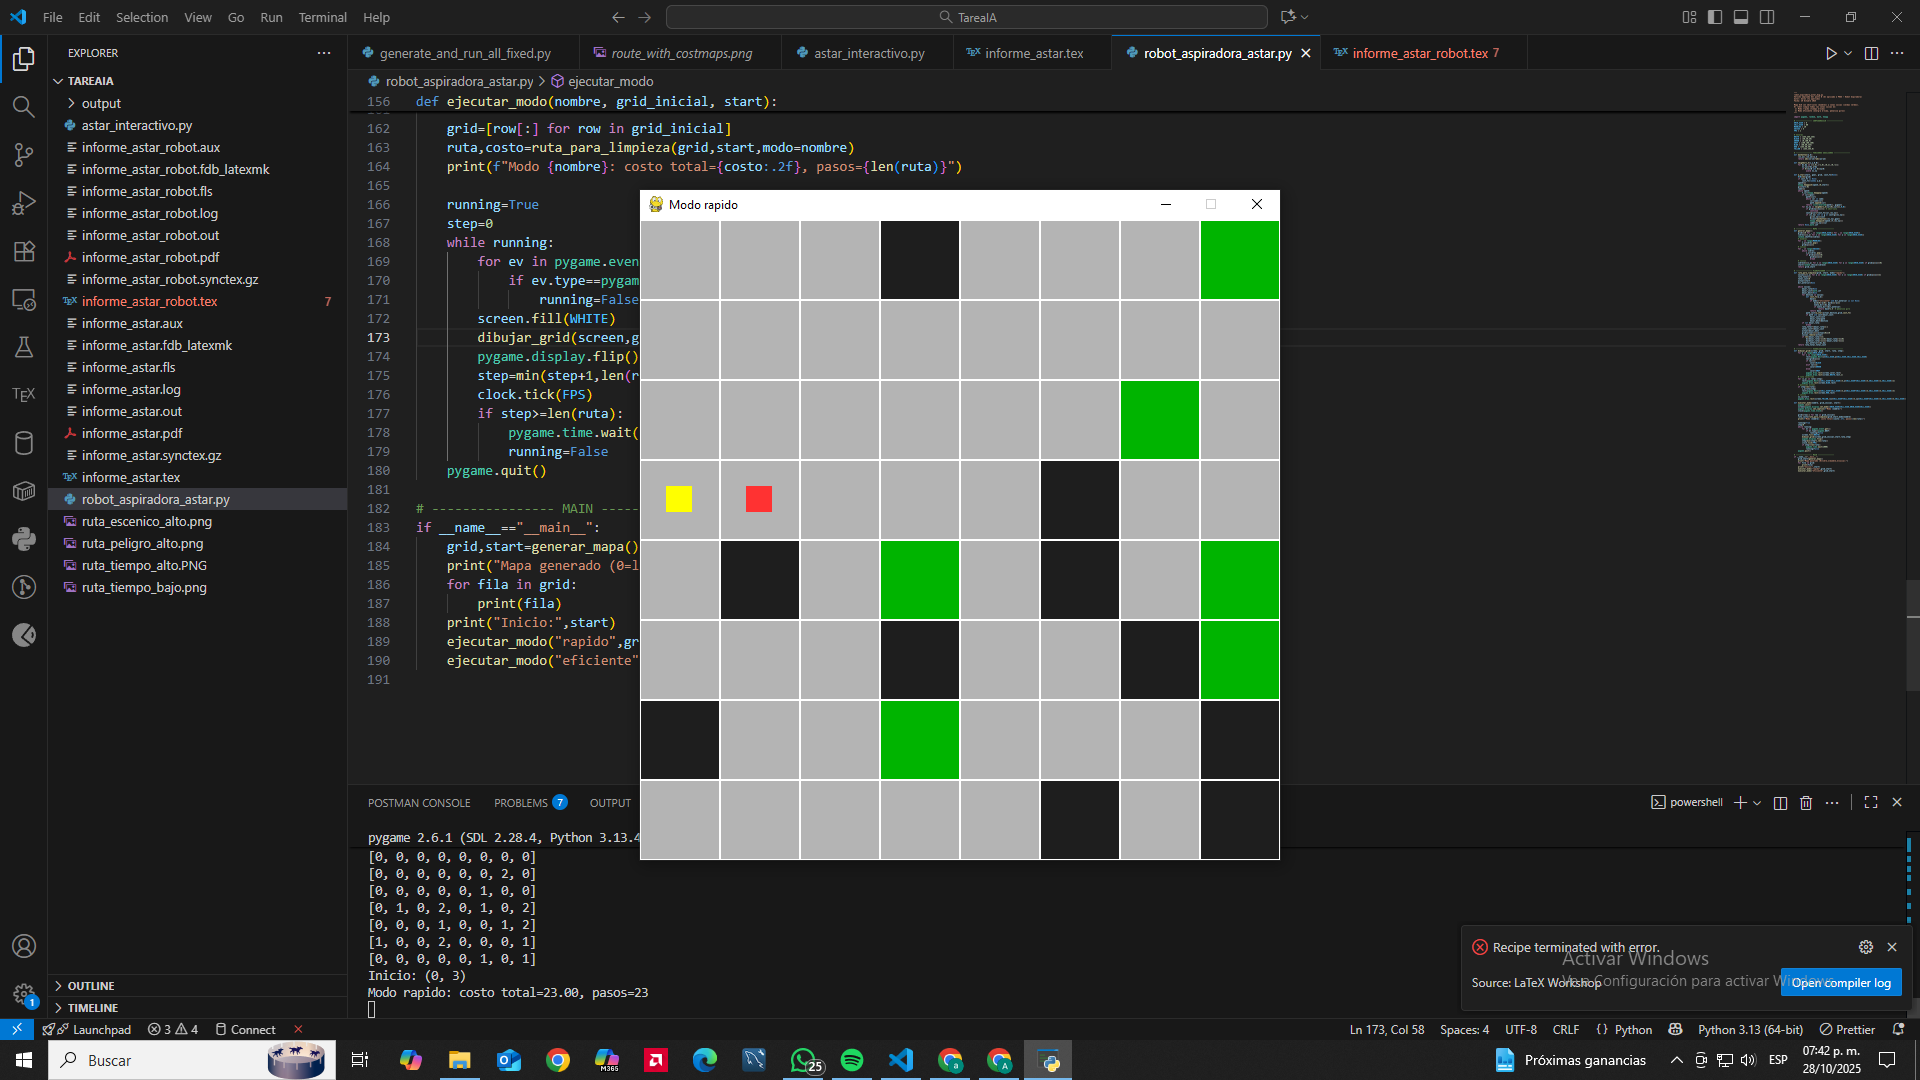
\includegraphics[width=0.65\textwidth]{mapa_inicial.png}
    \caption{Mapa inicial con obstáculos (negro), suciedad (verde) y posición inicial (amarillo).}
\end{figure}

%--------------------------------------------------
% MODOS DE OPERACIÓN
%--------------------------------------------------
\section{Modos de operación}

\subsection{Modo rápido}

En este modo, el robot calcula la secuencia de movimientos que minimiza el tiempo total de limpieza.  
No se consideran penalizaciones por cambio de dirección, por lo que tiende a girar más, pero termina antes.

\begin{figure}[H]
    \centering
    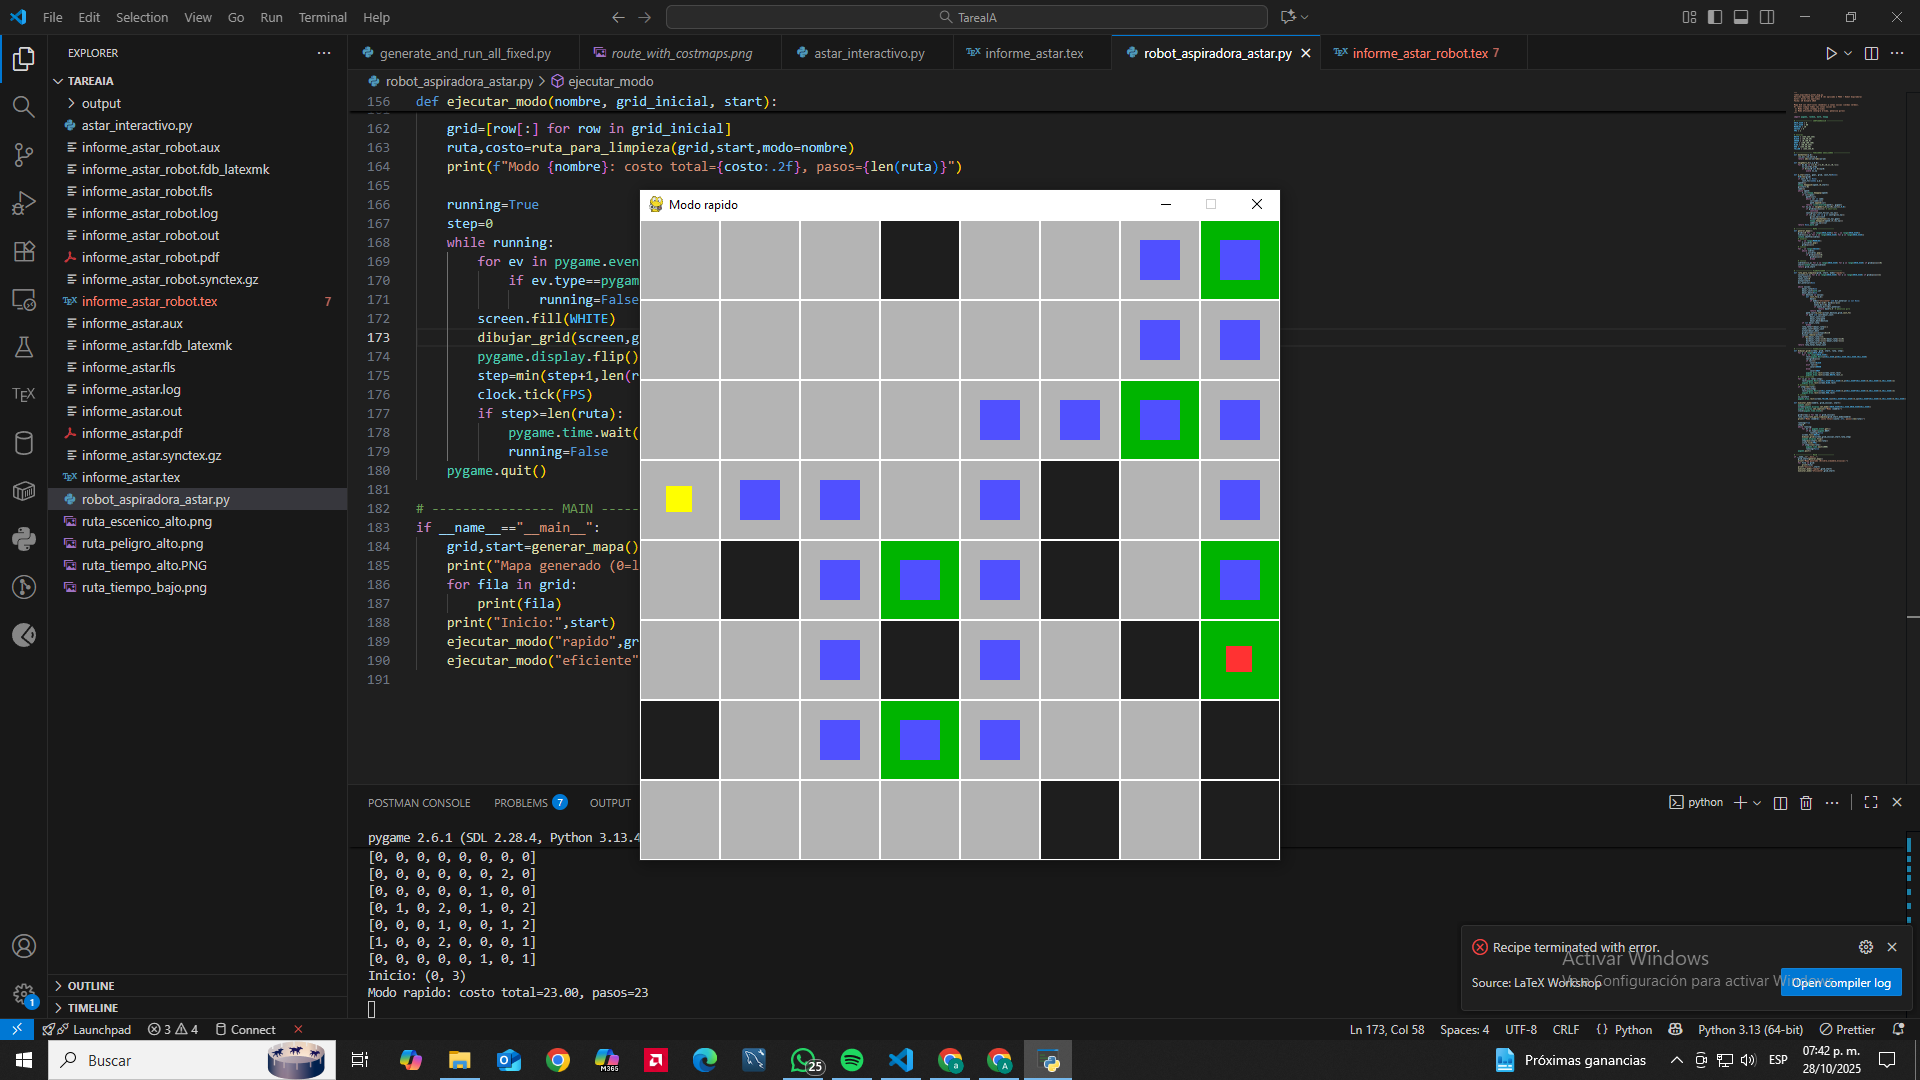
\includegraphics[width=0.8\textwidth]{ruta_rapida.png}
    \caption{Ruta obtenida en modo rápido. Se prioriza la distancia total mínima.}
\end{figure}

\subsection{Modo eficiente}

En este modo, el robot penaliza los giros con un costo adicional de $+1.5$ por cada cambio de dirección.  
Esto hace que busque trayectorias más suaves y rectas, reduciendo el gasto energético aunque aumente la distancia recorrida.

\begin{figure}[H]
    \centering
    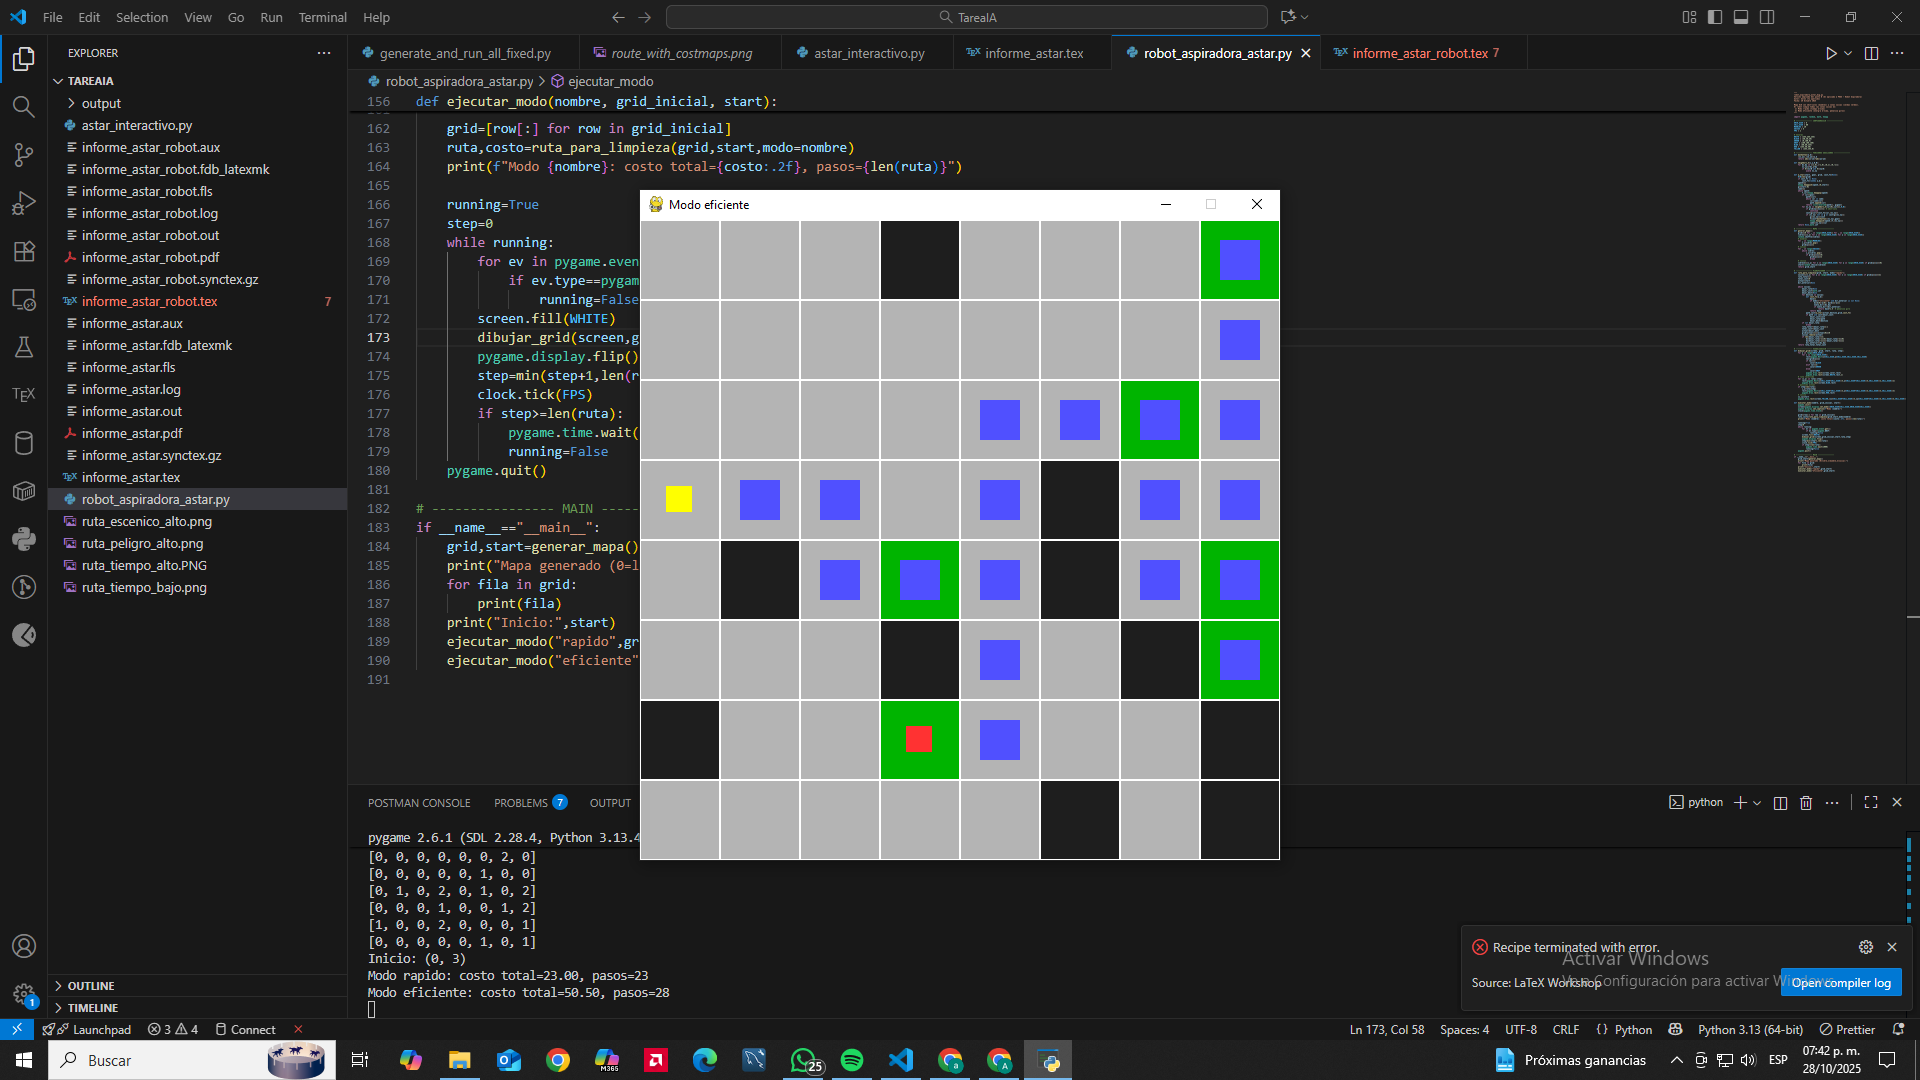
\includegraphics[width=0.8\textwidth]{ruta_eficiente.png}
    \caption{Ruta obtenida en modo eficiente. Se penalizan los giros y movimientos innecesarios.}
\end{figure}

%--------------------------------------------------
% COMPARACIÓN DE RESULTADOS
%--------------------------------------------------
\section{Comparación entre modos}

\begin{center}
\begin{tabular}{|c|c|c|}
\hline
\textbf{Modo} & \textbf{Costo total (A*)} & \textbf{Características observadas} \\
\hline
Rápido & Menor tiempo (menos pasos) & Más giros, mayor gasto energético. \\
\hline
Eficiente & Mayor tiempo & Menos giros, movimientos más directos. \\
\hline
\end{tabular}
\end{center}

La diferencia entre los modos es visible cuando el mapa tiene varios obstáculos:  
el modo rápido toma atajos, mientras que el modo eficiente elige trayectorias más suaves aunque sean más largas.

%--------------------------------------------------
% CONCLUSIONES
%--------------------------------------------------
\section{Conclusiones}

Este ejercicio demuestra cómo el algoritmo A* puede adaptarse a distintos criterios de optimización según la definición del modelo PEAS del agente.

\begin{itemize}
    \item En el modo rápido, el agente prioriza el \textbf{tiempo}, encontrando rutas más cortas pero con más giros.
    \item En el modo eficiente, el agente prioriza la \textbf{energía}, penalizando los giros y evitando trayectorias abruptas.
    \item El modelo PEAS permite definir formalmente el comportamiento inteligente del agente, separando los componentes de desempeño, entorno, sensores y actuadores.
\end{itemize}

En síntesis, este proyecto ilustra el uso de A* como base de un comportamiento racional adaptable a distintos objetivos dentro de un entorno simulado.

\vfill
\begin{center}
\textit{Fin del documento.}
\end{center}

\end{document}
